\documentclass[letterpaper,10pt]{article}
\usepackage[top=2cm, bottom=1.5cm, left=1cm, right=1cm]{geometry}
\usepackage{amsmath, amssymb, amsthm,graphicx}
\usepackage{fancyhdr}
\pagestyle{fancy}

\lhead{\today}
\chead{MV Stats Exam 3}
\rhead{Justin Hood}

\newcommand{\Z}{\mathbb{Z}}
\newcommand{\Q}{\mathbb{Q}}
\newcommand{\R}{\mathbb{R}}
\newcommand{\C}{\mathbb{C}}
\newtheorem{lem}{Lemma}

\begin{document}
\begin{enumerate}
\item We consider the data contained within Table 6.8 from the text. Here, we see data regarding the median times for a correct response when comparing the parity (odd or even) of numbers presented in both word, ("four"), and Arabic format, ("4"). We consider a repeated measures experiment with the design,
\begin{center}
\begin{tabular}{|l|l|l|}
\hline
& Different Parity & Same Parity\\\hline
Word Format & $X_1$ & $X_2$\\\hline
Arabic Format & $X_3$ & $X_4$\\\hline
\end{tabular}
\end{center}
This design is due to the fact that each of these variables $X_1, X_2, X_3, X_4$ are all measured for each of the 32 subjects, rather than say 4 different groups of 8 people. To begin our analysis, we compute the following,
\begin{align*}
\mu_1 &= \text{Mean Time for Word Format and Different Parity ``One/Two"}\\
\mu_2 &= \text{Mean Time for Word Format and Same Parity ``One/Three"}\\
\mu_3 &= \text{Mean Time for Number Format and Different Parity ``1/2"}\\
\mu_4 &= \text{Mean Time for Number Format and Same Parity ``1/3"}
\end{align*}
This can be represented as,
\[\mu = \begin{bmatrix}
967.5625\\875.6094\\825.3125\\710.9375
\end{bmatrix}\]
With these variables defined, we next consider the relevant contrasts between the variables. We want to test,
\begin{align*}
(\mu_3+\mu_4)-(\mu_1+\mu_2) &= \text{Test for diffrerence based on word/Arabic format}\\
(\mu_1+\mu_3)-(\mu_2+\mu_4) &= \text{Test for diffrerence based on same/different parity}\\
(\mu_1+\mu_4)-(\mu_2+\mu_3) &= \text{Test for interactions between Parity/Formatting}
\end{align*}
From this set of contrasts, we construct the matrix $C$ as,
\[C=\begin{bmatrix}
-1 & -1 & 1 & 1\\1 & -1 & 1 & -1\\ 1 & -1 & -1 & 1
\end{bmatrix} \]
From the original data, we also compute the covariance matrix,
\[S=\begin{bmatrix}
36178.35 \\
25936.73 & 22597.75 \\
18447.57 & 14261.73 & 18487.82 \\
15909.24 & 14115.93 & 11799.73 & 13001.40
\end{bmatrix} \]
as well as,
\[C\bar{x}=\begin{bmatrix}
-306.92188\\ 206.32812\\ -22.42188
\end{bmatrix};\ \ \ CSC'=\begin{bmatrix}
40269.292\\
-4799.164 & 19577.4776\\
-10403.748 & -987.1071 & 10007.3405
\end{bmatrix} \]
We consider the test,
\begin{align*}
H_0: & C\mu = \vec{0}\\
H_A: & C\mu \neq \vec{0}
\end{align*}
Here, $C\mu$ represents the value of the contrasts defined above. So, our null hypothesis assumes the difference between tests is zero.  To test for any differences between the different treatments, we compute,
\[T^2=n(C\bar{x})'(CSC')^{-1}(C\bar{x})=153.7275\]
as well as the critical test statistic,
\[T^*=\frac{(n-1)(q-1)}{n-q+1}F_{q-1,n-q+1}(\alpha)=9.40913\]
So, we see that $T^2>T^*$, and hence, we reject $H_0$ in favor of the alternative hypothesis. To see which of these contrasts are causing this difference, we consider the $95\%$ confidence intervals defined by,
\[c\bar{x} \pm \sqrt{\frac{(n-1)(q-1)}{n-q+1}F_{q-1,n-q+1}(\alpha)}\sqrt{\frac{c'Sc}{n}}\]
So, our intervals are,
\begin{align*}
(\mu_3+\mu_4)-(\mu_1+\mu_2) &= [-415.7364,\ -198.1074]\\
(\mu_1+\mu_3)-(\mu_2+\mu_4) &= [130.4567,\ 282.1995]\\
(\mu_1+\mu_4)-(\mu_2+\mu_3) &= [-76.6668,\ 31.82305]
\end{align*}
We note that zero is not within the first two intervals, i.e. the parity and format both have a nonzero effect on the outcome of the testing.\\
We are given that an absence of interaction supports the ``M" model of cognition while the presence of interaction supports the ``C and C" model. We see from our analysis that the third interval crosses zero. As such, we conclude that there does not appear to be any interaction in this data. Thus, our experimental analysis supports the ``M" model of numerical cognition.
\item We consider the data contained within Table 8.7 from the text. Here, we have data from 76 different farmers in West Africa on 9 different variables ranging from family size to number of goats on the farm. To begin our analysis, we look at scatter plots comparing the variables $X_1$ and $X_2$, as well as $X_2$ and $X_8$. These plots follow,
\begin{center}
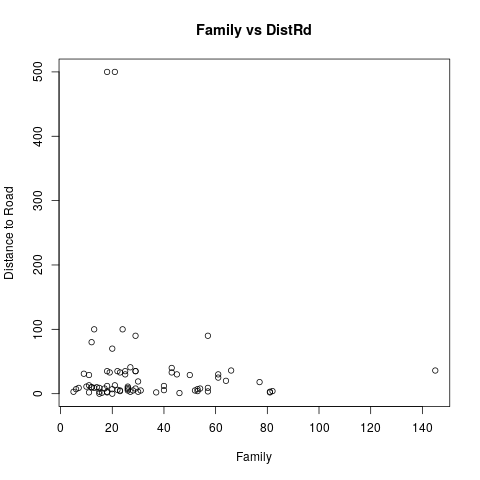
\includegraphics[scale=.5]{famdistscatter.png}
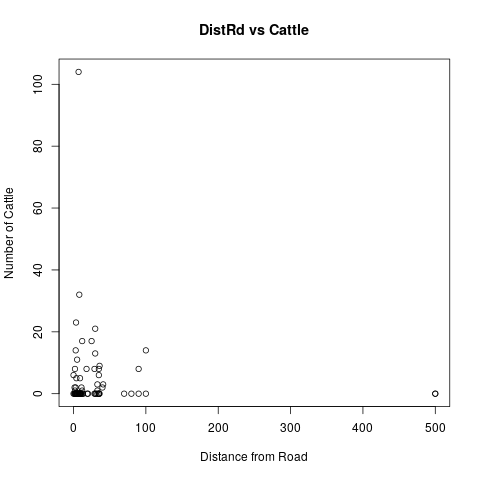
\includegraphics[scale=.5]{distcattlescatter.png}
\end{center}
From the first scatter,we see that there appear to be three outliers, two with large DistRd values, and one with large Family value. From the second, we see two outliers, with one large Cattle value, and one DistRd value. Using R, we find the list of offending cases to be,
\[Outliers = [25,\ 34,\ 69,\ 72]\]
So, we remove these rows from the data for the remainder of our analysis.\\
Next, we compute the correlation matrix $R$,
\[R=\begin{bmatrix}
1\\
-0.03148898 & 1\\
0.75684620 & -0.03110498 & 1\\
0.6552768 & 0.1098207 & 0.7157067 & 1\\
0.38803015 & -0.21839611 & 0.40686821 & -0.02987731 & 1\\
0.4964517 & -0.0832359 & 0.3520572 & 0.1756107 & 0.3638400 & 1\\
0.7333791  & 0.0283732 & 0.8213448 & 0.6289635 & 0.3181802 & 0.3362001 & 1\\
0.55328914 & 0.06006817 & 0.59865242 & 0.52986740 & 0.06017202 & 0.12529839 & 0.66980799 & 1\\
0.36173366 & 0.17095440 & 0.37260930 & 0.05091172 & 0.23713752 & 0.24981286 & 0.50378916 & 0.38185786 & 1
\end{bmatrix} \]
From this $R$ matrix, we perform an eigenvalue/vector computation, and make a scree chart from the magnitudes of the eigenvalues,
\begin{center}
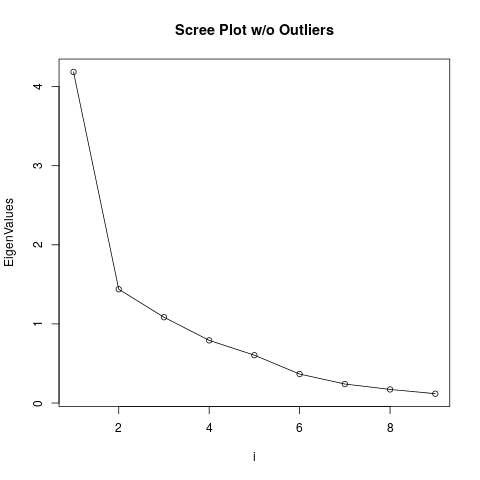
\includegraphics[scale=.5]{farmscree.png}
\end{center}
We see in the scree plot that there is a bend at the second point, but the magnitudes of the following values are still fairly large. Looking at the cumulative proportions of the eigenvalues, we see the following,
\[Cum\% = [0.4650146,\ 0.6248020,\ 0.7453020,\ 0.8332817,\ 0.9004289,\ 0.9411107,\ 0.9677800,\ 0.9868717,\ 1]\]
So, we see that the first five components cover 90\% of the variance, and the first six components cover 94\%. So, we conclude that five or six is probably the ideal number of components to use when summarizing the data.\\
Using the first five components, we look at the corresponding eigenvectors:
\[[e_1,\ e_2,\ e_3,\ e_4,\ e_5]=\begin{bmatrix}
0.433842713 & 0.065088695 & 0.09840025 & 0.17120143 & 0.01132705\\
0.007587031 & -0.496670914 & -0.56856059 & 0.49561039 & -0.37766811\\
0.446140316 & -0.008917253 & 0.13211700 & -0.02733684 & -0.21870789\\
0.352228405 & -0.352571495 & 0.38820350 & 0.24020492 & -0.07920345\\
0.203622111 & 0.603667416 & -0.11149246 & -0.05854254 & -0.64457738\\
0.240361102 & 0.415159516 & -0.11595977 & 0.61632679 & 0.52696668\\
0.445273680 & -0.068042477 & -0.03038787 & -0.14559178 & -0.02829987\\
0.355411548 & -0.284473439 & 0.01382636 & -0.37293370 & 0.21753184\\
0.254549533 & 0.048668251 & -0.68695528 & -0.35078804 & 0.24867109
\end{bmatrix} \]
Looking at the signs of the first vector, we see that they are all positive, as such this value is positively related to each of the variables. Since each of the variables measures the relative size or quantity of things on the farm, we see that this component could be considered an overall ``farm size" score. Looking to the second vector, we see that the positive values correspond to the DistRd, Sorgum, Millet, and Goats components. We see that the magnitudes of the Sorgum and Millet variables are large compared to the distance and goats variables, so we might consider this to be a measure of the farmland used for Sorgum and Millet compared to the remainder of the farm. Continuing, we see that the third component is of similar sign, however instead of the Sorgum and Millet, we are now looking at the Cotton and Maize farmland. Looking at the fourth vector's signs and magnitudes, we see that it might be considered a comparison of the rest of the farm to the number of animals on the farm. Finally, the fifth component is far more challenging to analyze. The values fall into the groupings,
\begin{align*}
+ &=[Family,\ Millet,\ Cattle,\ Goats]\\
- &=[DistRd,\ Cotton,\ Maize,\ Sorgum,\ Bull]
\end{align*}
At first glance, this appears to be a better analysis of the farming land vs the rest of the farm, but the magnitude of the Millet in the first group is large comparitively. This component could be treated as a measure of farming land less the millet vs. the rest of the farm, but that may not be a meaningful measure.
\item We now consider the data in the ``Creative Class" data set. To begin, we partition the data and isolate the rows of the data that correspond to the data from Wisconsin, Minnesota, North Dakota, South Dakota, and Michigan. We further partition the data and isolate only the counties of these states that are considered rural. Finally, we isolate the columns of the data that correspond to the variables ``CCShare" and ``BohShare", the proportion of jobs in the county that are classified as creative thinking and bohemian (arts) related. After our cleaning, we find that there are 47 entries for WI, 66 for MN, 49 for ND, 59 for SD, and 57 for MI, for a grand total of 278 entries total. From each of these states, we also compute the mean vectors and covariance matrices. These results follow,
\begin{align*}
WI: &\  \bar{x}=\begin{bmatrix}
0.1665047\\0.006677787
\end{bmatrix}\\
& S = \begin{bmatrix}
1.000697e-03 & 4.869107e-05\\
4.869107e-05 & 8.671019e-06
\end{bmatrix}\\
MN: &\  \bar{x}=\begin{bmatrix}
0.1718565\\ 0.007010424
\end{bmatrix}\\
& S = \begin{bmatrix}
1.150254e-03 & 2.771579e-05\\
2.771579e-05 & 1.308616e-05
\end{bmatrix}\\
ND: &\  \bar{x}=\begin{bmatrix}
0.1535318\\ 0.005158878
\end{bmatrix}\\
& S = \begin{bmatrix}
0.0009155548 & 2.208040e-05\\
0.0000220804 & 1.792505e-05
\end{bmatrix}\\
SD: &\  \bar{x}=\begin{bmatrix}
0.155181 \\ 0.00590178
\end{bmatrix}\\
& S = \begin{bmatrix}
1.919912e-03 & 8.549022e-05\\
8.549022e-05 & 3.858639e-05
\end{bmatrix}\\
MI: &\  \bar{x}=\begin{bmatrix}
0.1789028 \\ 0.007315439
\end{bmatrix}\\
& S = \begin{bmatrix}
1.101955e-03 & 7.162704e-05\\
7.162704e-05 & 1.899405e-05
\end{bmatrix}
\end{align*}
We see that the covariance matrices are all very similar in magnitude to eachother. As such, we test whether the covariances can be considered equal. We compute,
\[M = \left[\sum (n_l-1)\right]\ln|S_{pooled}|-sum[(n_l-1)\ln|S_l|]=53.61129\]
and,
\[u=\left[\sum\frac{1}{n_l-1}-\frac{1}{\sum(n_l-1)}\right]\left[\frac{2p^2+3p-1}{6(p+1)(g-1)}\right]=0.01614033\]
Then,
\[C=(1-u)M=52.74599\]
and,
\[C^*=21.02607\]
As such, we reject the null, that the covariances are equal, at the $\alpha=0.05$ level. Ordinarily we would stop our analysis, but we also note that for each state, we have a large value of $n$. As such, we feel safe in computing further, as the larger sample sizes will protect us from potential issues.\\
Continuing our analysis, we next compute,
\[W=\sum_{states} (n_{state}-1)S_{state}=\begin{bmatrix}
0.33780956 & 0.014070722\\
0.01407072 & 0.005411547
\end{bmatrix} \]
as well as,
\[\bar{x}=\frac{\sum_{states}n_{state}\bar{x}_{state}}{\sum_{states}n_{state}}=\begin{bmatrix}
0.165627518\\0.006455086
\end{bmatrix}\]
Finally, we compute,
\[B=\sum_{states}n_{state}(\bar{x}_{state}-\bar{x})(\bar{x}_{state}-\bar{x})'=\begin{bmatrix}
0.026249891 & 0.0019977844\\
0.001997784 & 0.0001652676
\end{bmatrix},\ \Lambda=\frac{|W|}{|W+B|}=0.9198643 \]
Now that we have computed our smaller scale values, we may compute our test statistic,
\[\left(\frac{\sum n-p-2}{p}\right)\left(\frac{1-\sqrt{\Lambda}}{\sqrt{\Lambda}}\right)=5.842908\]
and corresponding critical value,
\[T^*=3.353535\]
Hence, we see that at the $\alpha=0.01$ level, we reject the null hypothesis, that the proportions of jobs are the same between states, in favor of the alternative, that there is a difference between the states. To determine which states are different, we compute the simultaneous confidence intervals. All intervals are computed in R to be,
\begin{align*}
(WI-MN)_{CC} &= [-0.0243523,\ 0.01364864]\\
(WI-MN)_{Boh} &= [-0.002737493,\ 0.002072219]\\
(WI-ND)_{CC} &= [-0.007352348,\ 0.03329804]\\
(WI-ND)_{Boh} &= [-0.001053614,\ 0.004091434]\\
(WI-SD)_{CC} &= [-0.008139974,\ 0.0307873]\\
(WI-SD)_{Boh} &= [-0.001687471,\ 0.003239486]\\
(WI-MI)_{CC} &= [-0.03201259,\ 0.007216333]\\
(WI-MI)_{Boh} &= [-0.003120219,\ 0.001844916]\\
(ND-MN)_{CC} &= [-0.0370973,\ 0.0004479435]\\
(ND-MN)_{Boh} &= [-0.004227564,\ 0.0005244711]\\
(SD-MN)_{CC} &= [-0.03451173,\ 0.001160731]\\
(SD-MN)_{Boh} &= [-0.003366145,\ 0.001148856]\\
(MI-MN)_{CC} &= [-0.0109544,\ 0.02504698]\\
(MI-MN)_{Boh} &= [-0.001973302,\ 0.00258333]\\
(ND-SD)_{CC} &= [-0.02089046,\ 0.0175921]\\
(ND-SD)_{Boh} &= [-0.003178237,\ 0.001692432]\\
*(ND-MI)_{CC} &= [-0.0447648,\ -0.005977145]\\
(ND-MI)_{Boh} &= [-0.004611204,\ 0.0002980814]\\
*(SD-MI)_{CC} &= [-0.04221071,\ -0.005232868]\\
(SD-MI)_{Boh} &= [-0.003753769,\ 0.0009264514]
\end{align*}
We see that most of these CI's contain zero, but there are two, $(ND-MI)_{CC}$ and $(SD-MI)_{CC}$ that do not. As such, we see that these are the states and variable that are different amongst the Upper Midwest.
\item We consider the data from the VHA hospital records. To begin, we import the data and begin to clean it. Upon an initial inspection, we see that there are some rows in the data that are empty. As such, we shall remove these points from the analysis, since we do not want to artificially alter the data by adding zeros or the mean of the rest of the data. After this cleaning, we have $n=115$ observations, and $q=8$ data columns. This data includes standardized mortality rates from different conditions as well as statistics on patients time in the hospital vs the mean time. To begin our analysis, we compute the covariance matrix from the data. Looking at the data, we see that all of our entries are of relatively similar magnitudes, with the range of the data going from $-1.37$ to $95$. As such, we will compute our PCA on the $S$ matrix as opposed to the $R$ matrix. To start, we perform an eigen analysis on $S$, and make a Scree chart of the resultant eigenvalues.
\begin{center}
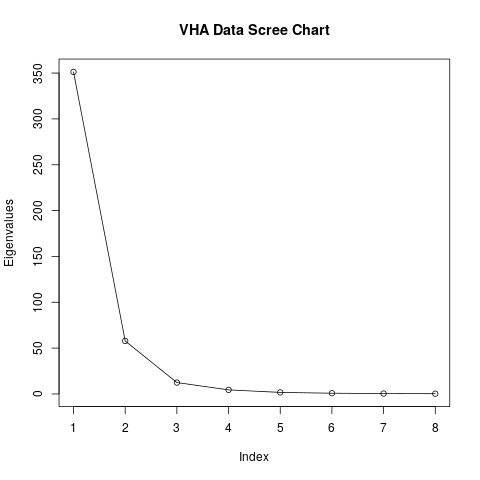
\includegraphics[scale=.5]{VHAscree.png}
\end{center}
We also see that the cumulative percentage of the variances are,
\[Cum\%=[0.8186629,\ 0.9533165,\ 0.9822214,\ 0.9925272,\ 0.9964436,\ 0.9983191,\ 0.9993317,\ 1]\]
We see that in the plot, there is a bend after around the third component. Looking at the corresponding percentages, we see that for the first three principle components, we can account for $98\%$ of the variance in the model. As such, we think that these components are probably an acceptable to model the data accurately for simpler analysis. We define three new variables, $v_1,\ v_2,\ v_3$ as,
\[v_1=\sqrt{\lambda_1}Xe_1,\ v_2=\sqrt{\lambda_2}Xe_2,\ v_3=\sqrt{\lambda_3}Xe_3\]
These new variables account for 98\% of the variance in the original data, while reducing the dimensionality of the data by 5 dimensions. As such, analysis and visualization will be much easier. Given that meaning can be drawn from each of these principle components, such as a measure of how effective the hospital is, these new variables can be plotted against eachother to discern higher meaning in a more visually appealing way.
\item Finally, we consider the Causes of Death dataset. We note that we may assume that the data may be cleaned and reorganized, and consider whether the following types of analysis may be useful.
\begin{enumerate}
\item First ANOVA/MANOVA. Given how the data is organized, we see that there are various ANOVA/MANOVA tests that may be run to glean more information on the data. Because we have two categorical variables, State and Cause of Death, we see that the data naturally falls into boxes that can be analyzed. Note, we assume that the Age-adjusted Death rate is linearly independent from the number of deaths, as the ages and other factors in this computation are independent state to state. So, now, we consider models, of the following form
\begin{center}
\begin{tabular}{l|l|l|l|l|}
& Cause 1 & Cause 2 & $\ldots$ & Cause $n$\\\hline
Alabama & $X_1, X_2$ &  $X_1, X_2$ & $\ldots$ & $X_1, X_2$\\\hline
Alaska & $X_1, X_2$ &  $X_1, X_2$ & $\ldots$ & $X_1, X_2$\\\hline
\vdots &&&&\\
Wyoming & $X_1, X_2$ &  $X_1, X_2$ & $\ldots$ & $X_1, X_2$\\\hline
\end{tabular}
\end{center}
where $X_1$ and $X_2$ are the death rate and age adjusted death rate respectively. We see here that a two way MANOVA can be used to compare these two variables between both states and the different causes themselves. Smaller and simpler ANOVA/MANOVAs can also be computed for different focuses of analysis. In order to perform these analyses, we also must assume that there are a large enough number of points for each dataset. Looking at the data, we see that the data has been collected over approximately 16 years, while we have the leading 10 causes of death. We see that each of the data vectors in our above model will have 11 points for each of the blocks, which should be sufficient for our purposes. We also assume that the data has been cleaned of any outliers that could throw off the analysis, as ANOVA is sensitive to these points. Finally, we also must first check that the death data is approximately MV normal, otherwise the analysis will fail. But for such large data sets, it should be acceptable to work on.
\item Next, we consider a PCA on the data that has been rearranged such that we have 10 columns corresponding to the causes of death. We consider whether PCA would provide valuable insight into the data. Thinking about the data, I do not think that PCA would provide any valuable information. Part of the assumptions that are used when doing the PCA is that somehow these variables can be combined in a meaningful way to reduce the number that we must work with. But, this also assumes that there is some dependency between them. Before, when we looked at the farming data, we saw that larger farms tended to have larger amounts of the various things that we were measuring, and so it makes sense to work on fewer variables for brevity. Here, we are considering our measured values to correspond to causes of death. These values are all inherently distinct, as we are only considering data on the underlying cause of death. So, looking at the data in the same way, for a state to have more deaths from a cause like stroke, we would not also assume that there was a positive or negative correlation that would propogate through the other causes of death in that state. I.e. it does not make sense to say that an increase in stroke deaths in WI would also increase the number of deaths due to cancer. As such, to perform a PCA, we would be forcing the data to take on meanings that are not necessarily valuable to us from an analysis perspective.
\item Next, we consider a Factor Analysis of the same cause data set. Because of factor analysis' basis in PCA, we will most likely not get any meaningful results from factor analysis either. But, we consider that factor analysis also has the ability to rotate the factors in such a way that the variables have a simpler structure. It is possible that there are groupings in the data that are not readily visible to us, especially since we do not have a strong background in the data itself. For example, it may come to light that a certain grouping of causes is inversely correlated to another, like (kidney disease and sepsis) vs. (alzheimers and suicide). Here, we see that the causes of death in each case are distinctly different, one doing with bacteria/viruses in the blood and organs, vs arguably issues with neurochemistry and psychology. By rotating the factors with respect to their optimal structure, FA has the potential to show us these groupings in a way that PCA could not. Given how the data would be structured in this case, we know that the causes of death are from continuous populations, and that there would be plenty of samples from all 50 states over 15 years. We also assume that outliers have been tested for and removed, a simple task with basic R libraries.
\item After looking at the above data, we see that we are most likely able to test for most simple statistics that we could wish to on the data. There is one type of analysis that should likely be computed as well, at the cause level, and that is a sense of a $T^2$ test. If the data is organized into the cause columns as described above, but then also scaled by either the total number of deaths, or the total for each cause, we can test to see whether there are distinct differences in our data from either previous data or assumptions, i.e. testing to see whether the \% of cancer deaths is over 25\% of the total deaths in a year. Another analysis that should be considered for the data as well is one of time scaling. Since we are measuring the data over the course of 16 years, it is possible, nay probable, that there are trends in the data. A cursory search online makes it clear that suicide rates have increased over the last 20 years, and it is easy to assume that other causes have seen changes over the years as well. As such, it is possible that data from the end of the study will overshadow or skew analysis differently than the earlier entries. By ignoring this shift, we are limiting the amount of useful data that can be extracted by our analyses. If we were to perhaps account for this time sensitive change in the data with some sort of regression scaling, the adjusted values could potentially be more useful than the data described above as is.
\end{enumerate}
\end{enumerate}
\end{document}
